\documentclass[tikz,border=5pt]{standalone}
\usepackage{fontspec}
\setmainfont{Times New Roman}
\usepackage{unicode-math}
\setmathfont{Cambria Math}
\usetikzlibrary{shapes.geometric,positioning,fit,arrows.meta,calc}

\begin{document}
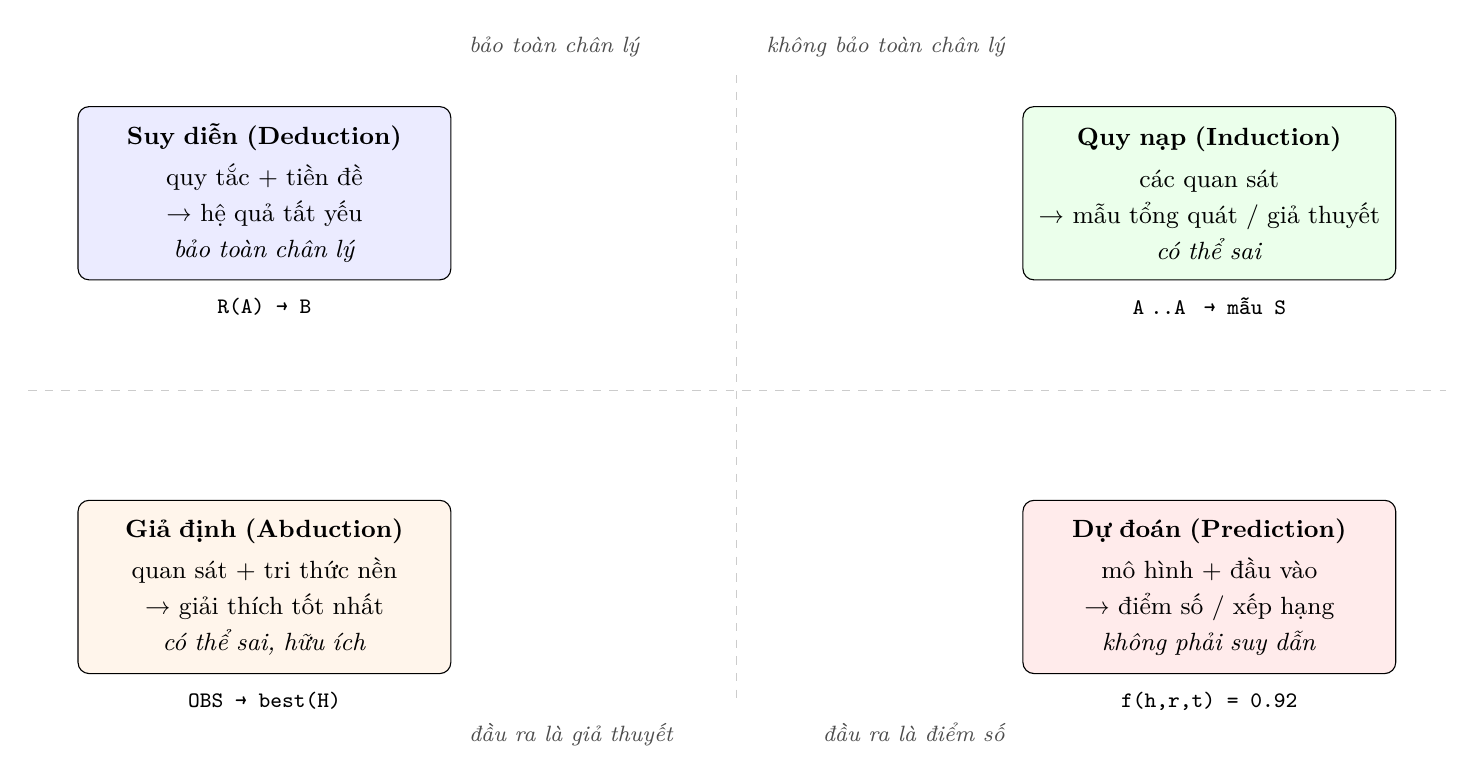
\begin{tikzpicture}[
  box/.style={rectangle, draw, rounded corners, align=center, text width=4.5cm, minimum height=2.2cm, font=\small},
  mono/.style={font=\footnotesize\ttfamily},
  label/.style={font=\footnotesize\itshape},
  arrow/.style={-{Stealth[length=2.5mm]}, thick},
  phase/.style={font=\footnotesize\bfseries},
]

\coordinate (C) at (0,0);

% === Deduction (top-left) ===
\node[box, fill=blue!8] (ded) at (-6, 2.5) {%
  \textbf{Suy diễn (Deduction)}\\[4pt]
  quy tắc + tiền đề\\[2pt]
  \textrightarrow\ hệ quả tất yếu\\[2pt]
  \textit{bảo toàn chân lý}
};
\node[mono, below=0.1cm of ded.south] {R(A) → B};

% === Induction (top-right) ===
\node[box, fill=green!8] (ind) at (6, 2.5) {%
  \textbf{Quy nạp (Induction)}\\[4pt]
  các quan sát\\[2pt]
  \textrightarrow\ mẫu tổng quát / giả thuyết\\[2pt]
  \textit{có thể sai}
};
\node[mono, below=0.1cm of ind.south] {A₁..Aₙ → mẫu S};

% === Abduction (bottom-left) ===
\node[box, fill=orange!8] (abd) at (-6, -2.5) {%
  \textbf{Giả định (Abduction)}\\[4pt]
  quan sát + tri thức nền\\[2pt]
  \textrightarrow\ giải thích tốt nhất\\[2pt]
  \textit{có thể sai, hữu ích}
};
\node[mono, below=0.1cm of abd.south] {OBS → best(H)};

% === Prediction (bottom-right) ===
\node[box, fill=red!8] (prd) at (6, -2.5) {%
  \textbf{Dự đoán (Prediction)}\\[4pt]
  mô hình + đầu vào\\[2pt]
  \textrightarrow\ điểm số / xếp hạng\\[2pt]
  \textit{không phải suy dẫn}
};
\node[mono, below=0.1cm of prd.south] {f(h,r,t) = 0.92};

% === Separators ===
\draw[dashed, gray!40] (0, 4) -- (0, -4);
\draw[dashed, gray!40] (-9, 0) -- (9, 0);

% === Axis labels ===
\node[label, text=gray!60!black, above right=0.5cm and 0.1cm of ded.north east] {bảo toàn chân lý};
\node[label, text=gray!60!black, above left=0.5cm and 0.1cm of ind.north west] {không bảo toàn chân lý};
\node[label, text=gray!60!black, below right=0.5cm and 0.1cm of abd.south east] {đầu ra là giả thuyết};
\node[label, text=gray!60!black, below left=0.5cm and 0.1cm of prd.south west] {đầu ra là điểm số};

\end{tikzpicture}
\end{document}